\documentclass[conference]{IEEEtran}
\usepackage{cite}
\usepackage{amsmath,amssymb,amsfonts}
\usepackage{graphicx}
\usepackage{array}
\usepackage{textcomp}
\usepackage{xcolor}
\usepackage[T1]{fontenc}
\usepackage{url}
\usepackage[hidelinks]{hyperref}
\def\IEEEkeywordsname{Keywords}
\pdfinfo{
  /Title (Replenish or Relieve: A Fog-to-Cloud Monitor for Footfall and Inventory Across a Two-Store Retail Floor)
  /Author (Adithya Reddy Madireddy)
}

\begin{document}

\title{Replenish or Relieve: A Fog-to-Cloud Monitor for Footfall and Inventory Across a Two-Store Retail Floor}

\author{\IEEEauthorblockN{Adithya Reddy Madireddy}
\IEEEauthorblockA{Student ID: X25120280 \\ MSc in Cloud Computing \\ Fog and Edge Computing (H9FECC) \\ National College of Ireland \\ x25120280@student.ncirl.ie}}

\maketitle

\begin{abstract}
A shop loses money in two opposite directions at once, and a manager has to watch both. A shelf that runs empty, a chiller that drifts warm, and a checkout queue that builds all cost the store, but they are not the same kind of problem: an empty shelf is a shortfall to be topped up, while a warm fridge, a long queue, and a crowded floor are pressures to be relieved. This project builds a monitor that reads both directions across a two-store floor and decides which is which at the edge. Five signals, footfall, shelf stock, refrigeration temperature, queue length, and energy draw, are read from ten sensor processes across the two stores; a fog gateway on the in-store host windows each store-and-signal stream, reduces it to a summary, and evaluates a small set of retail rules whose direction is chosen to match the operation, a lower bound on stock that says replenish and upper bounds on temperature, queue, and crowding that say relieve, with energy carried alongside as context rather than as an alarm. A serverless backend on Amazon SQS, AWS Lambda, and Amazon DynamoDB persists the summaries, and a store operations board served through Amazon API Gateway folds the latest window of every store into estate-wide totals a manager can read at a glance, with the static frontend delivered from Amazon S3. The awkward part of the edge tier is concurrency: ten posting threads share one window while a timer empties it, and rather than guard that buffer with a lock the design gives it to a single owner thread reached only through a mailbox, so a flush is just another message and can never interleave with a write. The system was provisioned to a real Amazon Web Services account rather than to a local emulator; a suite of 122 automated tests passes, and verification against the live endpoint confirmed both stores streaming all five signals, the board rolling them into estate totals, and the checkout-congestion rule firing on the stores whose queues had built.
\end{abstract}

\begin{IEEEkeywords}
retail analytics, inventory monitoring, footfall, fog computing, edge computing, Internet of Things, serverless computing, Amazon SQS, AWS Lambda, Amazon DynamoDB
\end{IEEEkeywords}

\section{Introduction}

Retail runs on attention that does not scale. A store manager can walk the floor, glance at the chillers, and judge the checkout queues, but only a few times an hour and only for one store at a time, and the losses that matter accumulate in the gaps between those walks. A shelf that empties mid-morning sells nothing until someone notices it; a refrigerated case that drifts warm puts its stock at risk long before the next inspection; a queue that builds at the tills turns shoppers away in minutes. Each of these is a continuous quantity that a periodic human check samples far too coarsely, and the connected store answers by instrumenting those quantities and watching them without pause \cite{caro2019, gubbi2013}.

What makes the retail case interesting as a data problem is that the signals do not all fail in the same direction. Shelf stock is a quantity that hurts when it falls: the alarm is a lower bound, and the response is to replenish. Refrigeration temperature, queue length, and footfall are quantities that hurt when they rise: the alarm is an upper bound, and the response is to relieve, by servicing a chiller, opening a till, or easing crowding. A monitor that treats every signal as a ceiling to stay under would miss the emptying shelf entirely, so the rule layer here is built around the direction of each signal rather than a single comparison applied uniformly. A fifth signal, energy draw, is carried without an alarm at all, because on its own it names no fault; it is context that helps explain the others, since a hot afternoon lifts footfall and refrigeration load together.

The distributed-systems question is where the watching happens. The Internet of Things makes it cheap to place a sensor on every shelf, case, and doorway \cite{atzori2010}, but streaming every raw reading from every store to a distant cloud region to be judged there is wasteful in two directions. It spends bandwidth continuously on readings that, taken singly, rarely change a decision, and it defers the one moment that matters, a signal crossing its threshold, until after a network round trip. Fog computing was proposed to close that gap by placing a compute tier between the sensors and the cloud, near enough to summarise, filter, and evaluate rules before anything travels \cite{bonomi2012, yousefpour2019}, and it is one expression of the broader movement of computation back toward the network edge \cite{shi2016, satyanarayanan2017}. Behind that edge tier, the cloud supplies the elastic, pay-as-used model that removes the need to size a server for a peak that is idle most of the day \cite{armbrust2010}.

This project builds that two-tier design for a scaled but faithful slice of a retail estate: two stores, designated store-1 and store-2, each carrying the same five signals, run as ten independent sensor processes. A fog gateway on the in-store host receives their readings, groups each store-and-signal pair into a fixed time window, reduces the window to summary statistics, evaluates the retail rules against the summary, and forwards only the finished window and any alert it raises. A serverless cloud pipeline persists each window, and a store operations board folds the persisted history into an estate view that shows each store against its signals and rolls the whole floor into the few totals a manager acts on.

The work pursues four objectives, each shown on a running system rather than only described. The first is a sensor and fog layer that genuinely windows and evaluates five heterogeneous retail signals at sampling and dispatch rates that are configurable rather than fixed in code. The second is a backend that scales through managed, elastic AWS primitives instead of a single always-on server. The third is a board that turns stored windows into an operating read a manager could act on without inspecting raw values. The fourth, and the one that separates a working system from a plausible one, is deployment onto a real public-cloud account and verification against the live endpoint. Scope is held to these layers at a two-store scale rather than a whole chain. The remainder of this paper is organised as follows. Section~II presents the architecture and the reasoning behind each choice, including the alternatives weighed and the security posture. Section~III covers the implementation, the automated tests, continuous integration, the real deployment, and the evidence gathered from the running system. Section~IV closes with a critical assessment of the trade-offs, the limits, and where the work could go next.

\section{System Architecture and Design}

Fig.~\ref{fig:topology} shows the deployed system end to end: ten sensor processes and the fog gateway sharing one in-store host, a managed queue, two independently deployed functions, a key-value store, and a browser-facing bucket reached through a managed gateway.

\begin{figure*}[!t]
\centering
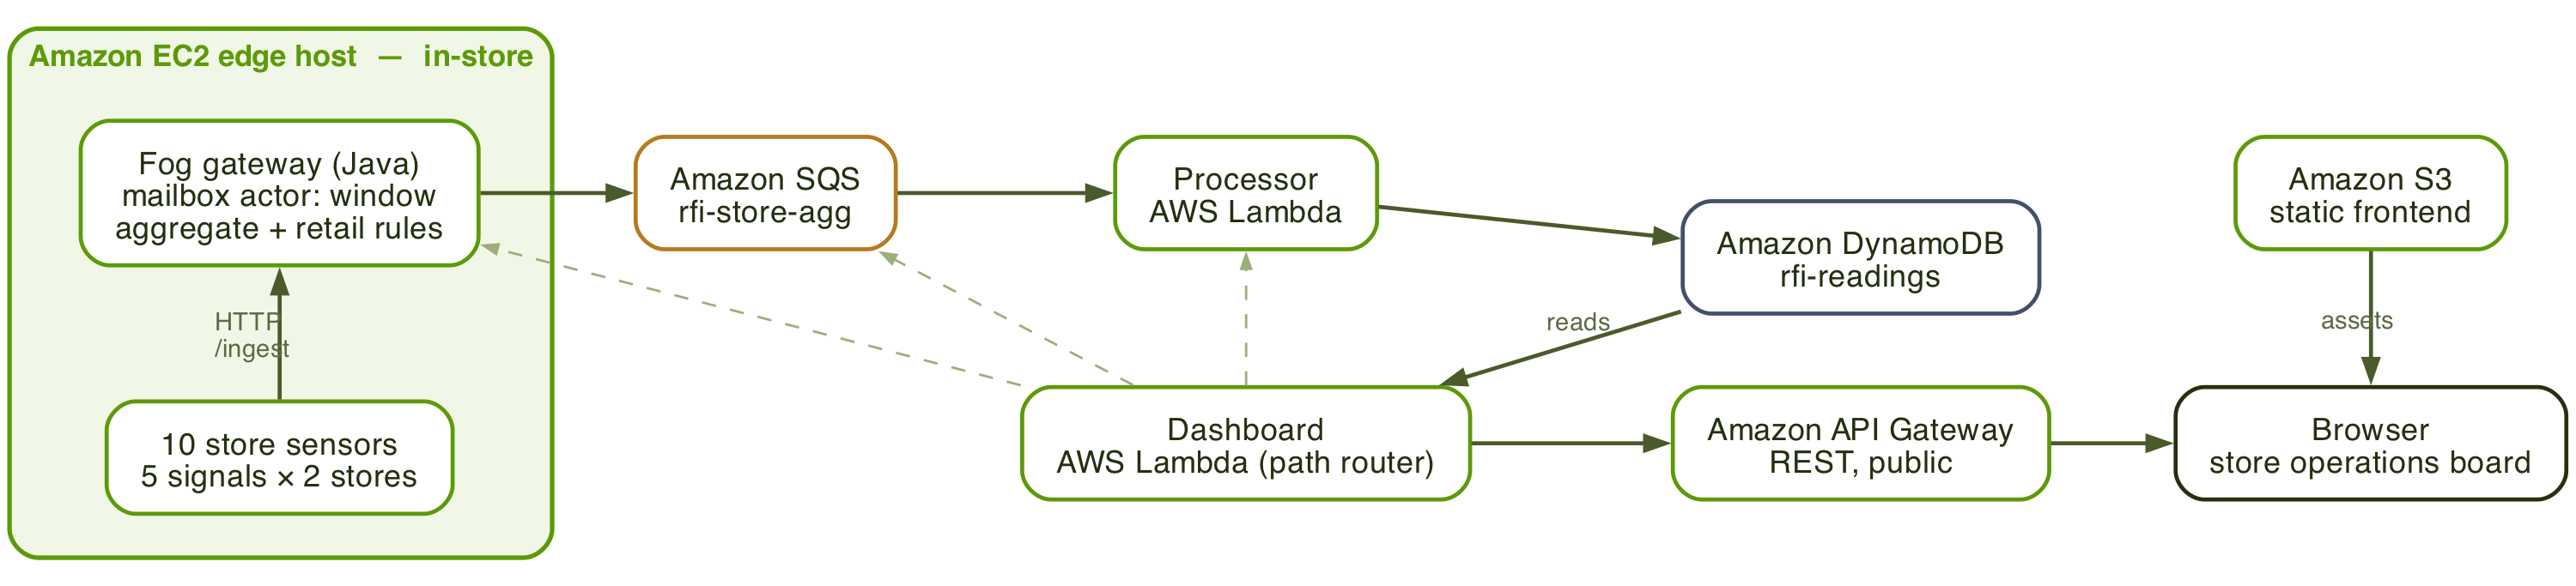
\includegraphics[width=0.95\textwidth]{topology.png}
\caption{Deployment topology. Ten sensor processes and the fog gateway share one Amazon EC2 host inside the store. Solid arrows are the ingest path, from the fog gateway through Amazon SQS and the processor function into the Amazon DynamoDB table, and the serving path, from the dashboard function's read of the stored windows out through Amazon API Gateway to the browser, with static assets from Amazon S3. The dashed edges are the three further status sources the board polls for its health strip: the fog gateway's reachability, the queue's depth, and the processor function's deployment state.}
\label{fig:topology}
\end{figure*}

\subsection{Sensor and Fog Layer}

Each of the ten sensor processes represents one signal in one store. On every sampling tick a process advances a bounded random walk: it nudges its previous value by a step drawn uniformly from a small symmetric range and clamps the result into a plausible band for that signal, so consecutive readings stay close together like a real feed rather than independent noise. The bands differ sharply by signal, and that difference is the heterogeneity the design has to carry: footfall sits in the low hundreds of visitors, shelf stock is a percentage, refrigeration temperature runs in a narrow band around a few degrees, queue length is a small count of people, and energy draw is in the tens of kilowatts. A process samples on one interval and dispatches on another, and the two are independent so a fast-moving quantity can be sampled often while still being shipped in economical batches; the sampling interval defaults to two seconds and the dispatch interval to ten. On each dispatch the accumulated readings are posted as a compact JSON object naming the signal, the store, and the unit and carrying the batch of values gathered since the last dispatch, which at the default rates is roughly five readings amounting to a few hundred bytes on the wire, well under a kilobyte. The process posts it over HTTP to the fog gateway's ingest endpoint, so the input interface is an ordinary HTTP call the sensors make rather than a shared file or a direct write to storage.

The fog gateway is a Java service that serves its ingest endpoint on the runtime's own built-in HTTP server rather than a web framework, keeping the edge component dependency-light, and it runs as its own container on the in-store host distinct from the sensor processes and the cloud functions. It does real work before anything leaves the store. The centre of the gateway is a single-owner buffer, and the reasoning behind it is the awkward part of the whole edge tier. Readings arrive on the built-in server's handler pool, which is several threads at once, while a scheduled task has to seal the window on a fixed timer; the two touch the same buffer, and the usual answer is a lock. This design takes a different route: one dedicated worker thread owns the buffer outright, and every other thread reaches it only by posting a message into a queue that the worker drains in order. An arriving reading becomes a message the handler thread drops and returns from immediately; the window close becomes another message, a request for a snapshot and reset, that the worker answers by handing back the sealed window and starting an empty one. Because the close is just another message in the same single-consumer queue, it can never run in the middle of a write, so the loss of a reading landing exactly on a window boundary is not guarded against but designed out.

When a window closes, each non-empty store-and-signal group is reduced to a summary carrying the count, minimum, maximum, average, and latest value, and that summary, not any raw reading, is evaluated against the retail rules. The rules are held as a small set of typed entries, each a signal, the comparison it applies, its limit, and the alert it raises, and a single evaluation reads the named field from the summary and fires the alert when the comparison holds. This structure is what lets the rules follow the direction of each signal rather than a fixed template. Shelf stock is the one signal tested on a lower bound: when its window average falls under the floor the gateway raises a restock alert, because the fault is depletion and the response is to top the shelf up. The other three alarmed signals are tested on upper bounds, because their fault is pressure and the response is to relieve it: refrigeration temperature above its ceiling raises a cold-chain warning, queue length above its ceiling raises a checkout-congestion alert, and footfall above its ceiling raises a capacity warning. Energy draw is summarised and shown but carries no rule at all, a deliberate choice to keep it as context that explains the others rather than a fault in its own right. The same rule set is grouped by signal and served verbatim on a thresholds endpoint, so the board can disclose the limits without the disclosure ever driving evaluation.

The fog gateway's output interface is a real managed queue rather than a direct write to storage. On each window boundary it batches the closed summaries and sends them to Amazon SQS in grouped calls, each carrying up to the service's per-call limit of ten summaries, so a busy cycle costs a number of send operations proportional to the summaries closing divided by ten rather than one send per summary. At start-up it resolves the queue's address once, retrying while the queue is still being provisioned, because on a fresh deployment the queue may not exist when the in-store host boots, and a failed send is logged and the cycle continues rather than crashing the gateway, a bias toward keeping the edge live that suits a monitoring workload where the next window is only seconds away.

\subsection{Backend Layer}

The cloud tier follows a single ingest path with a branch for the operator interface. A queue receives the fog gateway's summaries, one function drains the queue and writes to storage, and a second, separately deployed function reads that storage back to answer the board. Splitting the write path from the read path is deliberate: ingestion and querying then scale and fail independently, so a surge of windows cannot slow the board and a burst of manager activity cannot back up ingestion.

\textit{Queue instead of a direct call.} The fog gateway could invoke the storage function directly and synchronously, dropping the queue and saving a hop. That option was declined. A synchronous call binds the edge to the availability and latency of the cloud function: throttle it, leave it cold, or take it down briefly, and the fog gateway stalls or sheds data as the back-pressure propagates toward the sensors. A queue severs that coupling, absorbs bursts, retries on the consumer's behalf, and lets the gateway treat a summary as delivered the moment it is enqueued \cite{hohpe2003}. On a ten-second cadence the small added latency is immaterial, while the decoupling and durability are exactly what an intermittent in-store link needs.

\textit{Event-driven functions instead of a standing server.} Both the ingestion and the interface tiers run as event-driven functions. This fits work that arrives in bursts and, for the interface, only intermittently: billing is per request rather than for idle capacity, and the platform adds and removes instances as demand shifts, with nothing reserved up front \cite{armbrust2010}. The recognised cost is the cold start after a period of idleness \cite{wang2018}; its effect here is small, because steady queue traffic keeps the ingestion function warm and the board's own polling keeps the interface function warm. The processor function is triggered by the queue, holds no state between invocations, and is billed only for the work it does. It reads a batch of queued summaries, folds each into a stored record, and attempts every message in the batch even when one is malformed, failing the batch back to the queue only at the end so that a single bad record cannot discard its healthy neighbours while the queue's own redelivery retries the failure.

\textit{Key-value store instead of a relational database.} A relational engine would offer joins and open-ended queries, neither of which this workload uses. Its access pattern is narrow and known in advance: append summaries in time order, then fetch the most recent windows for a given signal. Amazon DynamoDB, an on-demand key-value store built for that mix of heavy writes and key-based reads, holds its performance as the table grows and spares the operational overhead of running a relational server, the balance the original Dynamo work set out and the managed service now carries \cite{decandia2007, elhemali2022}. The key design follows straight from the query. Each stored window is keyed on its signal as the partition and on a sort value that leads with the window's closing timestamp and then the store identifier, so windows for one signal are already ordered chronologically inside a single partition and the newest are read with one bounded, descending, single-partition query rather than a scan; the store in the sort tail keeps the two stores' windows distinct within the same signal.

\subsection{Serving Layer and Security Posture}

The board reaches the read function through a managed gateway that publishes a public REST endpoint. Object storage holds the static frontend, one page, a stylesheet, the page script, and a charting library kept in the repository rather than pulled from a content-delivery network. The read function keeps one set of query and health helpers that both a local server and the deployed function share; run locally it is served from the runtime's built-in HTTP server, and as a deployed function it is a small router that maps each gateway request path to the matching helper, since the local server's socket binding has no meaning inside a function. It exposes a small, read-only surface: a stores endpoint giving each store's latest window per signal, a readings endpoint returning a recent series for one signal, a thresholds endpoint that forwards the gateway's published rules, a backend-statistics endpoint, and a health endpoint assembled from four live sources, the store for the freshest window, the queue for its reachability, the processor function for its deployment state, and the fog gateway for its reachability, returning a pipeline flag that is true only when a window actually reached the store in the last thirty seconds. The backend-statistics endpoint reports the total number of stored windows, and because a count over the whole table can exceed a single response page, it follows the store's pagination contract and walks every page rather than trusting the first, so the figure stays correct as the table grows.

The board is built around the estate view rather than a single store. Above the per-store detail it computes, live on each read from the latest window of every store, the few totals a manager actually acts on: the footfall across the whole floor, the count of stores currently understocked, the average checkout queue, and the total energy draw. Below that, each store is a card showing its five signals with a current value, a recent range, and any alert currently firing, and a small trend line tracks each signal across recent windows for both stores together. A banner names any firing alert by store and signal, and a health strip along the top reports the four pipeline indicators in plain green or red. A fixed browser-side timer re-fetches the estate summary, health, and statistics every 2.5 seconds and repaints from whatever the responses hold, so the view stays current without a manual reload and without any server-push channel. The page learns which gateway origin to call from a single placeholder written into it and substituted with the real endpoint when the assets are uploaded; run locally, where one process serves both the page and the interface, the placeholder resolves to empty and requests fall back to the same origin. The security posture is modest and deliberate for a scaled demonstration: the fog gateway's health and threshold endpoints answer without a credential check because they expose only aggregate window state and configured limits, never a live per-sensor reading, while the cloud tier relies on the managed services' own access control and on scoping each function to the queue, table, and gateway it needs.

\section{Implementation}

The system is organised as four independent Java modules on the Java~17 runtime, one each for the sensor process, the fog gateway, the processor function, and the dashboard function, so that a change in one is built and tested on its own and the tiers never share mutable state through a common library. The fog gateway serves its ingest, health, and threshold endpoints on the runtime's built-in HTTP server rather than a web framework, keeping the edge component dependency-light; JSON is handled with Jackson in the fog gateway and both backend functions, with the sensor process emitting its small fixed payload directly, and the AWS SDK for Java carries the queue, table, and function calls. The sensor process and the fog gateway are packaged as containers and run on the in-store host, while the processor and dashboard modules are built as function artefacts and deployed as event-driven functions; the frontend renders its trends with a locally kept charting library so the page has no external dependency at load time. The edge tier is orchestrated with Docker Compose, the cloud tier is provisioned with Terraform, and continuous integration runs on GitHub Actions.

The retail rules and the aggregation are kept in the fog module as plain data and pure functions, which is what makes the edge tier both testable and cheap to extend. A rule is a typed entry of a signal, a comparison, a limit, and an alert name, and the rules for the four alarmed signals sit in one grouped set; adding a new alert, or giving a signal a different direction, is a new entry in that set rather than a new branch in a growing conditional, and because the evaluation reads the named field from an already-computed summary it never re-scans the raw readings. The aggregation is likewise a single pass over the window that yields the count, extremes, average, and latest value in one traversal, so the cost of closing a window is linear in the readings it holds and independent of how many rules will later consult the summary.

\subsection{Testing and Continuous Integration}

The system carries an automated suite of 122 tests, fifty-six over the sensor process including a fifty-iteration repeated check that the bounded walk never leaves its band, twenty-eight over the fog gateway, twenty-four over the dashboard function, and fourteen over the processor function. They run without any cloud connection by exercising the units against hand-written fake AWS clients, so each test can assert on the exact shape of the request a given call would issue rather than depending on a live service. The fog tests are pointed where the risk is: the window aggregation arithmetic on known inputs, the batched relay's chunking at the queue's per-call limit, and each retail rule at and around its limit, with shelf stock checked just inside and just outside its lower floor and the three ceiling rules checked the same way, so that the direction of every rule is pinned down rather than assumed. The dashboard tests are the densest after the sensor's repeated check, because the deployed function's request routing is code the local server never runs and so is the part most exposed to a deployment-only mistake: they cover the per-store estate assembly from stored windows, the recent-series query that feeds the trends, the four health checks including the page-walking record count that must stay correct across a multi-page table, and the path routing the function performs against a gateway event. The processor tests cover the folding of a queued summary into a stored record, including the composite sort value that orders windows within a partition and the batch that keeps its healthy records when one message is malformed. The sensor tests cover the bounded walk staying inside its band and the payload it encodes. The suite runs on every push through GitHub Actions, so a change that breaks a rule boundary, a batch size, a query shape, or the routing fails in continuous integration rather than after deployment.

Testing against fakes rather than a live queue was a deliberate choice with a cost worth acknowledging: a fake asserts on the request a call would make, not on how the managed service behaves under load, so the batched-send limit and the queue's own retry semantics were reasoned about from the service documentation \cite{awssqs} and then confirmed against the live deployment rather than in unit tests.

\subsection{Deployment and Live Verification}

The cloud tier was provisioned to a real AWS account in a single Terraform apply that created twenty-four resources, with the account confirmed before anything was applied and the working state isolated so the apply could add only its own resources and never disturb anything already present. Describing the whole cloud tier as code, rather than clicking it together once, means the same definition builds the queue, both functions with their triggers and permissions \cite{awslambda}, the table, the gateway with its single catch-all route \cite{awsapigw}, and the two buckets in one reproducible step, and tears them down as cleanly. The in-store host runs the fog gateway and the ten sensor containers under Docker Compose; the deployed resources carry a common prefix so the deployment is easy to identify and remove as a unit, the public dashboard bucket is named for the store operations board it serves, and a fixed public address in front of the in-store host lets the read function reach the gateway's health and threshold endpoints at the same location across restarts.

Verification was carried out against the live deployment rather than a local emulator, and Fig.~\ref{fig:dashboard} is the deployed board during that check. Within about a minute of start-up the pipeline reported healthy end to end: the fog gateway, the queue, the processor function, and the freshest-window recency all read healthy, and the newest window was a few seconds old on each poll. Both stores rendered all five signals with their current value and recent range; the estate row folded the two stores into a live floor total, a count of understocked stores, an average queue, and a total energy draw, all of which moved across successive polls rather than staying static; and the alert banner correctly named a checkout-congestion alert on the stores whose queue length had built past its ceiling, while leaving the depletion floor and the refrigeration ceiling unflagged, which is the direction-aware rule set doing exactly what a single uniform comparison could not. Reaching the board from a browser also exercised the cross-origin path from the storage bucket to the gateway, which returned data cleanly.

\begin{figure}[!t]
\centering
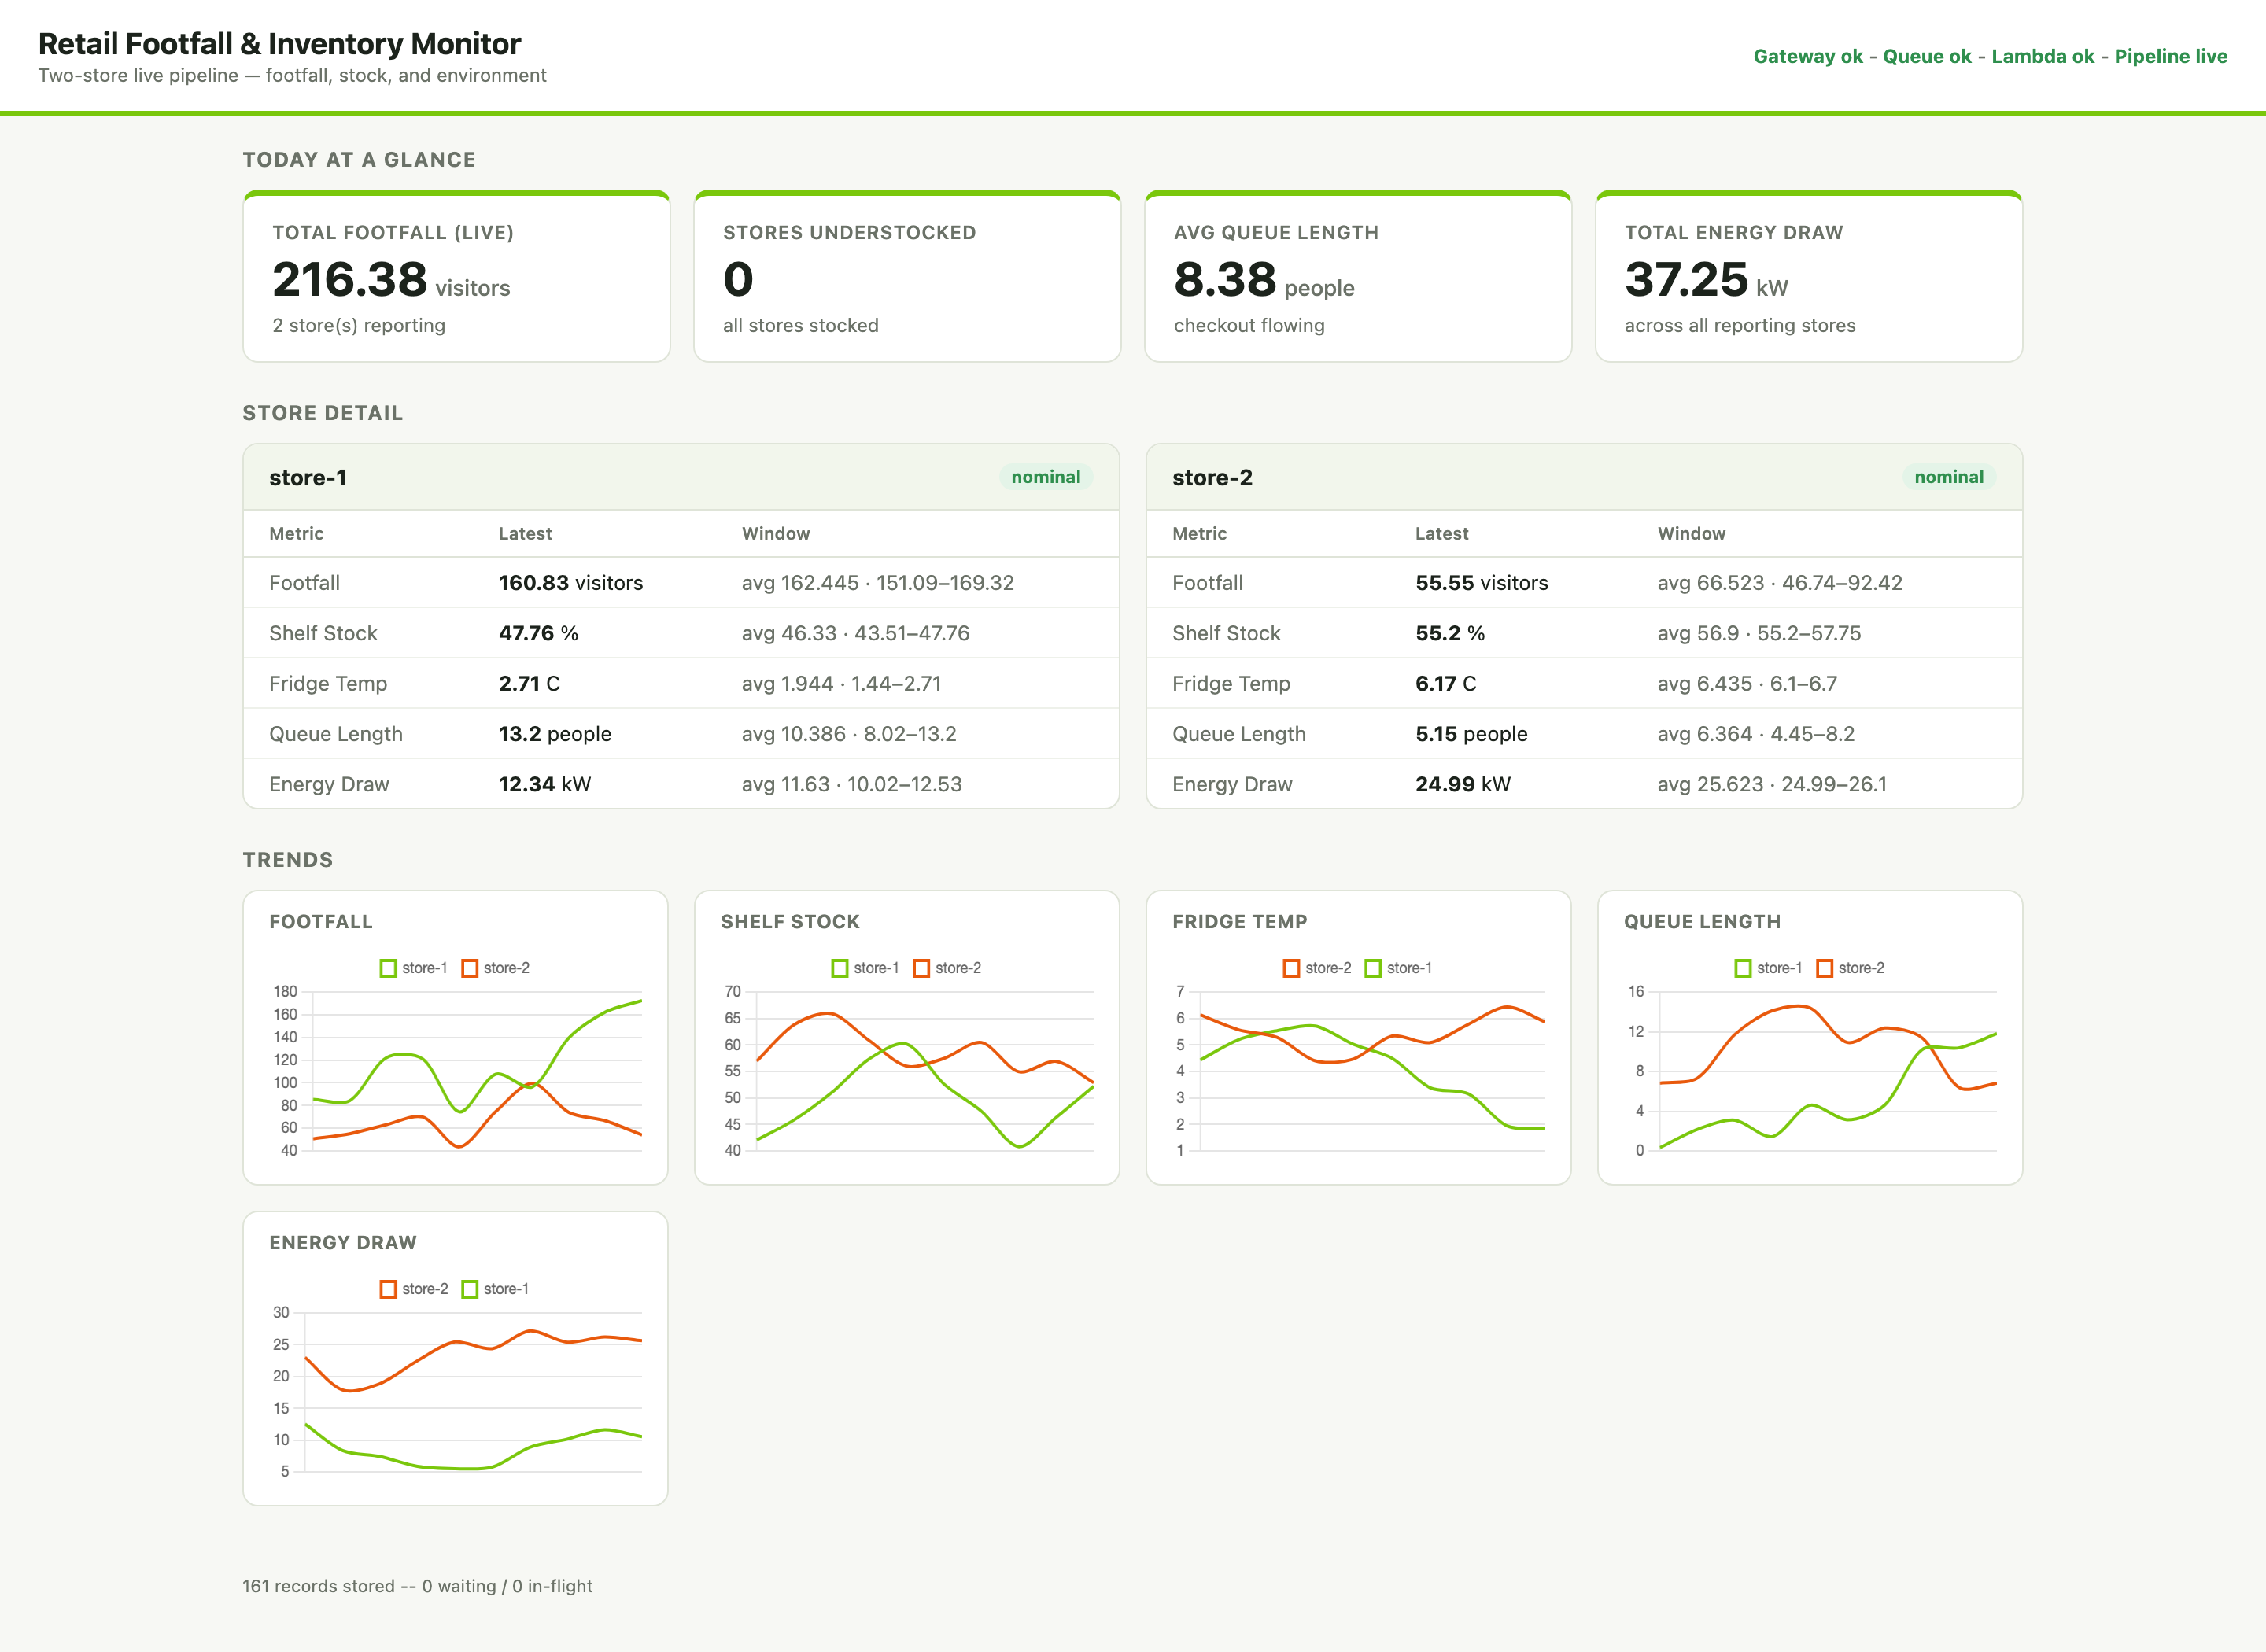
\includegraphics[width=\columnwidth]{dashboard.png}
\caption{The deployed store operations board reading from the live endpoint. The estate row folds both stores into a live floor total, an understocked-store count, an average queue, and a total energy draw; each store card shows its five signals against their current value and recent range; the trend charts track each signal across recent windows for both stores; the banner names any firing alert by store; and the health strip shows the four pipeline indicators in green.}
\label{fig:dashboard}
\end{figure}

\section{Conclusion}

This project set out to build and, above all, to deploy a fog-to-cloud pipeline that turns five retail signals across two stores into an operating read a manager can act on, and it met that goal on a running system rather than on paper. The edge tier does genuine work before anything travels: it windows and reduces each store-and-signal stream and evaluates the retail rules locally, so only compact summaries cross the network and an alert is named in the window it appears. The cloud tier scales through decoupling and elasticity rather than a pre-sized server, using a queue to absorb bursts and separate the write and read paths, event-driven functions billed only for the work they do, and an on-demand key-value store whose key design turns the board's one query into a single-partition read. The whole system was provisioned to a real account by one infrastructure-as-code apply and verified end to end against the live endpoint, with 122 automated tests guarding its behaviour and continuous integration running them on every change.

Building the system taught two lessons worth recording. The clearer one is that a retail floor cannot be watched with a single kind of rule. A ceiling suits the pressures, a queue that has to be relieved, a case that has to be cooled, a doorway that must not overfill, but the shelf is the mirror image: its fault is emptiness, so it has to be alarmed as it falls, and the fifth signal, energy, earns no rule at all because on its own it accuses nothing. Letting each signal choose its own direction, and letting the result surface as an estate roll-up rather than a wall of separate gauges, is what turned raw numbers into the two verbs a manager actually uses, replenish and relieve. The subtler lesson is about the shape of the concurrency rather than a guard placed around it. The obvious way to let many posting threads and one flushing timer share a buffer is to wrap the buffer in a lock; the route taken here instead gives the buffer a single owner and lets everyone else reach it only by leaving a message, so the flush becomes one more message in the same line and the window boundary has no gap in which a reading can be lost. Removing the possibility, rather than defending against it, is what kept the busy ingest path uncontended and made the missing-reading case something the design cannot express rather than something it merely avoids.

The work has clear limits. It runs at a two-store scale with simulated signals, its rule limits are fixed rather than learned from each store's own baseline or adjustable at runtime, and its security posture is intentionally modest for a demonstration. Natural next steps are to widen it to many stores and real sensor feeds, to move the fixed limits to a managed configuration a manager could tune per store without a redeploy, to add authentication and a custom domain in front of the public endpoint, and to retain longer history so a slow drift, a shelf that empties a little earlier each day, can be trended rather than only alarmed. None of these changes the shape of the pipeline, which is the point: the edge-aggregation and cloud-serving design carries from two stores to many without rethinking the tiers.

\begin{thebibliography}{00}
\bibitem{caro2019} F. Caro and R. Sadr, ``The Internet of Things (IoT) in Retail: Bridging Supply and Demand,'' \emph{Business Horizons}, vol. 62, no. 1, pp. 47--54, 2019.
\bibitem{gubbi2013} J. Gubbi, R. Buyya, S. Marusic, and M. Palaniswami, ``Internet of Things (IoT): A Vision, Architectural Elements, and Future Directions,'' \emph{Future Generation Computer Systems}, vol. 29, no. 7, pp. 1645--1660, 2013.
\bibitem{atzori2010} L. Atzori, A. Iera, and G. Morabito, ``The Internet of Things: A Survey,'' \emph{Computer Networks}, vol. 54, no. 15, pp. 2787--2805, 2010.
\bibitem{bonomi2012} F. Bonomi, R. Milito, J. Zhu, and S. Addepalli, ``Fog Computing and Its Role in the Internet of Things,'' in \emph{Proc. MCC Workshop on Mobile Cloud Computing}, 2012, pp. 13--16.
\bibitem{yousefpour2019} A. Yousefpour et al., ``All One Needs to Know about Fog Computing and Related Edge Computing Paradigms: A Complete Survey,'' \emph{Journal of Systems Architecture}, vol. 98, pp. 289--330, 2019.
\bibitem{shi2016} W. Shi, J. Cao, Q. Zhang, Y. Li, and L. Xu, ``Edge Computing: Vision and Challenges,'' \emph{IEEE Internet of Things Journal}, vol. 3, no. 5, pp. 637--646, 2016.
\bibitem{satyanarayanan2017} M. Satyanarayanan, ``The Emergence of Edge Computing,'' \emph{Computer}, vol. 50, no. 1, pp. 30--39, 2017.
\bibitem{armbrust2010} M. Armbrust et al., ``A View of Cloud Computing,'' \emph{Communications of the ACM}, vol. 53, no. 4, pp. 50--58, 2010.
\bibitem{hohpe2003} G. Hohpe and B. Woolf, \emph{Enterprise Integration Patterns: Designing, Building, and Deploying Messaging Solutions}. Addison-Wesley, 2003.
\bibitem{wang2018} L. Wang, M. Li, Y. Zhang, T. Ristenpart, and M. Swift, ``Peeking Behind the Curtains of Serverless Platforms,'' in \emph{USENIX Annual Technical Conference}, 2018, pp. 133--146.
\bibitem{decandia2007} G. DeCandia et al., ``Dynamo: Amazon's Highly Available Key-value Store,'' in \emph{Proc. ACM SIGOPS Symp. Operating Systems Principles}, 2007, pp. 205--220.
\bibitem{elhemali2022} M. Elhemali et al., ``Amazon DynamoDB: A Scalable, Predictably Performant, and Fully Managed NoSQL Database Service,'' in \emph{USENIX Annual Technical Conference}, 2022, pp. 1037--1048.
\bibitem{awssqs} Amazon Web Services, ``Amazon Simple Queue Service Developer Guide,'' 2024. [Online]. Available: \url{https://docs.aws.amazon.com/sqs/}
\bibitem{awslambda} Amazon Web Services, ``AWS Lambda Developer Guide,'' 2024. [Online]. Available: \url{https://docs.aws.amazon.com/lambda/}
\bibitem{awsapigw} Amazon Web Services, ``Amazon API Gateway Developer Guide,'' 2024. [Online]. Available: \url{https://docs.aws.amazon.com/apigateway/}
\bibitem{ieeetemplate} IEEE, ``Manuscript Templates for Conference Proceedings,'' 2024. [Online]. Available: \url{https://www.ieee.org/conferences/publishing/templates.html}
\end{thebibliography}

The source code and deployment configuration are available at [GitHub repository URL].

\end{document}
